\documentclass[11pt]{article}
\usepackage[a4paper,margin=2.2cm]{geometry}
\usepackage{pgfplots}
\pgfplotsset{compat=1.18}
\usepackage{amsmath}
\usepgfplotslibrary{statistics}
\usepackage{booktabs}
\usepackage{array}
\usepackage{longtable}
\usepackage[table]{xcolor}
\usepackage{hyperref}
\usepackage{titlesec}
\usepackage{caption}
\usepackage{float}
\usepackage{enumitem}
\hypersetup{colorlinks=true,linkcolor=teal,urlcolor=blue!60!black}
\titleformat{\section}{\Large\bfseries\color{teal!70!black}}{}{0em}{}[\titlerule]
\titleformat{\subsection}{\large\bfseries\color{blue!60!black}}{}{0em}{}

\definecolor{supacol}{HTML}{3ECF8E}
\definecolor{r2col}{HTML}{F38020}
\definecolor{warn}{HTML}{B00020}

\title{\textbf{Cost Scaling Report}\\ \large Poultry-Training App on Supabase + Cloudflare R2\\ \normalsize When the free tier breaks, and what 1k\,$\to$\,10M users cost}
\author{Generated \today}
\date{}

\begin{document}
\maketitle

\begin{abstract}\small
This report models the monthly running cost of the \emph{poultry-training} chat \& inquiry app as its user base grows from 1 to 10\,M registered accounts. The stack is \textbf{Supabase} (Postgres, Auth, Realtime, Edge Functions, Storage) on the \textbf{Pro} plan plus \textbf{Cloudflare R2} for media (inquiry videos/images). All numbers come from the live pricing pages of Supabase\footnote{\url{https://supabase.com/pricing}} and Cloudflare R2\footnote{\url{https://developers.cloudflare.com/r2/pricing/}}, computed by the model in \texttt{docs/cost-analysis/cost-model.js}. Graphs are drawn with \texttt{pgfplots}.
\end{abstract}

\section{Pricing facts used (Pro plan + R2)}

\begin{table}[H]\centering\small
\caption{Supabase Pro plan quotas and overage rates (monthly).}
\begin{tabular}{l r r l}
\toprule
\textbf{Line item} & \textbf{Included} & \textbf{Over rate} & \textbf{Unit} \\
\midrule
Plan subscription        & ---            & \$25 flat     & /org/month \\
Compute (Micro)         & \$10 credit    & \$10--\$3,730  & /instance \\
Auth MAU                 & 100{,}000      & \$0.00325     & /MAU \\
Egress (uncached)        & 250 GB         & \$0.09        & /GB \\
Cached egress            & 250 GB         & \$0.03        & /GB \\
Disk / DB size           & 8 GB           & \$0.125       & /GB \\
File storage             & 100 GB         & \$0.0213      & /GB \\
Edge Function invocations& 2{,}000{,}000  & \$2.00        & /1M inv \\
Realtime peak connections& 500            & \$10.00       & /1k conn \\
Realtime messages        & 5{,}000{,}000  & \$2.50        & /1M msg \\
\bottomrule
\end{tabular}
\end{table}

\begin{table}[H]\centering\small
\caption{Cloudflare R2 pricing (Standard storage). \textbf{Egress is free.}}
\begin{tabular}{l r r l}
\toprule
\textbf{Line item} & \textbf{Free tier} & \textbf{Rate} & \textbf{Unit} \\
\midrule
Storage                & 10 GB-month    & \$0.015  & /GB-month \\
Class A ops (writes)   & 1{,}000{,}000  & \$4.50   & /1M req \\
Class B ops (reads)    & 10{,}000{,}000 & \$0.36   & /1M req \\
Egress to Internet     & \multicolumn{2}{l}{\textbf{Free}} & \\
\bottomrule
\end{tabular}
\end{table}

\section{When does the free tier stop being enough?}

The app is on the \textbf{Free} plan today. The hard limits that will break it first, in order of likelihood:

\begin{enumerate}[leftmargin=*]
\item \textbf{Database size \textgreater{} 500 MB} $\Rightarrow$ the project enters \emph{read-only mode} (no new messages/inquiries). This is the first wall: with the modeled row sizes, $\approx$\,\textbf{12{,}000 active users} (or $\sim$6 months of retained messages for $\sim$2{,}000 MAU) fills 500 MB.
\item \textbf{Egress \textgreater{} 5 GB/month} $\Rightarrow$ the trainee page polls ``message from trainer'' every 5\,s. With $\sim$\,\textbf{250 DAU} each spending 8 min/day, poll egress alone crosses 5 GB.
\item \textbf{Realtime \textgreater{} 200 concurrent connections} $\Rightarrow$ hit at roughly \textbf{120--150 simultaneous} online users.
\item \textbf{Edge Functions \textgreater{} 500k invocations} $\Rightarrow$ crossed around \textbf{600--800 MAU} because of the polling endpoint.
\item \textbf{Auth \textgreater{} 50{,}000 MAU} and \textbf{Storage \textgreater{} 1 GB} $\Rightarrow$ media uploads (R2 is used, so this rarely bites).
\item \textbf{Free projects pause after 1 week of inactivity} — fine for a hobby, fatal for production SLA.
\end{enumerate}

\textbf{Recommendation:} move to \textbf{Pro (\$25/mo)} as soon as you exceed \emph{any} of: 500 MB DB, 5 GB egress, $\sim$150 concurrent realtime users, or you need the app to never pause. Everything below assumes the Pro plan.

\section{Workload model assumptions}

The figures are driven by per-user behaviour typical of the trainee chat/inquiry app:

\begin{itemize}[leftmargin=*,itemsep=2pt]
\item 40\% of registered accounts are monthly active; 35\% of those are daily active.
\item Each active trainee: $\sim$200 chat messages/month, $\sim$10 inquiries/month (one media each, 50/50 video\,/\,image, 3 MB video and 150 KB image compressed).
\item Each active trainee page polls the ``message from trainer'' endpoint every 5\,s during an 8-minute session, $\sim$12 sessions/month $\Rightarrow$ \textbf{polling is the dominant egress + Edge Function driver}.
\item Postgres keeps $\sim$6 months of messages/inquiries; R2 keeps 12 months of media.
\item Compute size is bumped by DAU and DB size (Micro $\to$ 16XL).
\end{itemize}

\section{Cost breakdown by user band}

\begin{table}[H]\centering\scriptsize
\caption{Monthly cost (USD). \texttt{Base} = Pro \$25 + compute; \texttt{Usage} = Supabase metered overages; \texttt{R2} = Cloudflare media.}
\begin{tabular}{r l r r r r r r r r r r}
\toprule
\textbf{Users} & \textbf{Compute} & \textbf{DB} & \textbf{Egress} & \textbf{EdgeFn} & \textbf{Auth} & \textbf{RT} & \textbf{SupBase} & \textbf{SupUsage} & \textbf{SupTotal} & \textbf{R2} & \textbf{TOTAL} \\
\midrule
1           & Micro  & 0.0  & 0.0   & 0      & 0    & 0   & 25  & 0.0   & 25.0  & 0.0    & 25.0    \\
50          & Micro  & 0.0  & 0.0   & 0      & 0    & 0   & 25  & 0.0   & 25.0  & 0.0    & 25.0    \\
500         & Micro  & 0.2  & 0.0   & 0      & 0    & 0   & 25  & 0.0   & 25.0  & 0.4    & 25.4    \\
1{,}000     & Micro  & 0.5  & 0.0   & 0      & 0    & 0   & 25  & 0.0   & 25.0  & 0.9    & 25.9    \\
\rowcolor{yellow!20} 10{,}000 & Small  & 4.7  & 0.0 & 1.2 & 0   & 3.4 & 30  & 4.6   & 34.6  & 10.7   & 45.3    \\
100{,}000   & Large  & 47.1 & 0.0   & 48.1   & 0    & 86.1& 125 & 139.1 & 264.1 & 108.4  & 372.4   \\
1{,}000{,}000 & 2XL  & 471  & 170   & 517    & 975  &1019 & 425 & 2738  & 3163  & 1104   & 4266    \\
10{,}000{,}000 & 8XL & 4711 & 1898  & 5202   & 12675& 10343&1885& 30706& 32591 & 11113  & 43703   \\
\bottomrule
\end{tabular}
\end{table}

\subsection{The headline numbers}

\begin{table}[H]\centering
\caption{Total monthly cost vs. registered users (log scale).}
\begin{tabular}{r r r}
\toprule
\textbf{Registered users} & \textbf{\$/month} & \textbf{\$/user/month (active)} \\
\midrule
1{,}000       & \$26     & \$0.065 \\
10{,}000      & \$45     & \$0.011 \\
100{,}000     & \$372    & \$0.0093 \\
1{,}000{,}000 & \$4{,}266& \$0.0107 \\
10{,}000{,}000& \$43{,}703& \$0.0109 \\
\bottomrule
\end{tabular}
\end{table}

The cost per active user flattens around \textbf{\$0.01} once you are past a few thousand users — the model is dominated by metered usage (polling egress, Edge Functions, DB size), and doubling users roughly doubles the bill. The floor is the \$25 Pro subscription + a compute instance.

\section{Charts}

\subsection{Total monthly cost vs.\ users (log--log)}

\begin{figure}[H]\centering
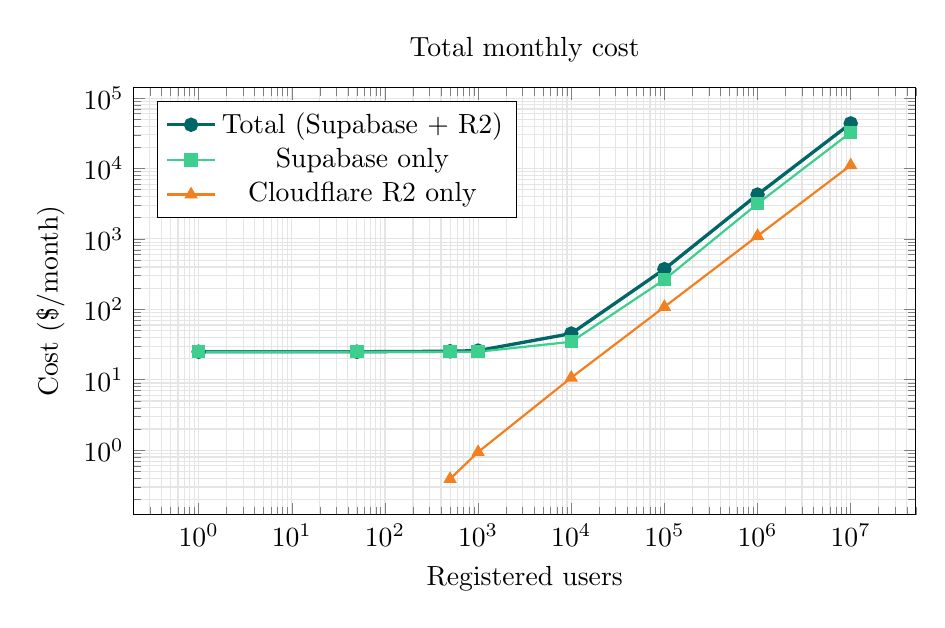
\begin{tikzpicture}
\begin{loglogaxis}[
  width=0.95\textwidth, height=7cm,
  xlabel={Registered users}, ylabel={Cost (\$/month)},
  legend pos=north west, grid=both, grid style={gray!20},
  title={Total monthly cost},
]
\addplot[color=teal!80!black, very thick, mark=*] coordinates {
  (1,25) (50,25) (500,25.39) (1000,25.94) (10000,45.31) (100000,372.42) (1000000,4266.40) (10000000,43703.30)
};
\addlegendentry{Total (Supabase + R2)}
\addplot[color=supacol, thick, mark=square*] coordinates {
  (1,25) (50,25) (500,25) (1000,25) (10000,34.61) (100000,264.05) (1000000,3162.57) (10000000,32590.68)
};
\addlegendentry{Supabase only}
\addplot[color=r2col, thick, mark=triangle*] coordinates {
  (1,0) (50,0) (500,0.39) (1000,0.94) (10000,10.70) (100000,108.38) (1000000,1103.84) (10000000,11112.61)
};
\addlegendentry{Cloudflare R2 only}
\end{loglogaxis}
\end{tikzpicture}
\caption{Log--log cost curve. R2 (orange) grows roughly linearly with media volume; Supabase (green) jumps when compute and metered overages kick in.}
\end{figure}

\subsection{Cost composition by user band (stacked)}

\begin{figure}[H]\centering
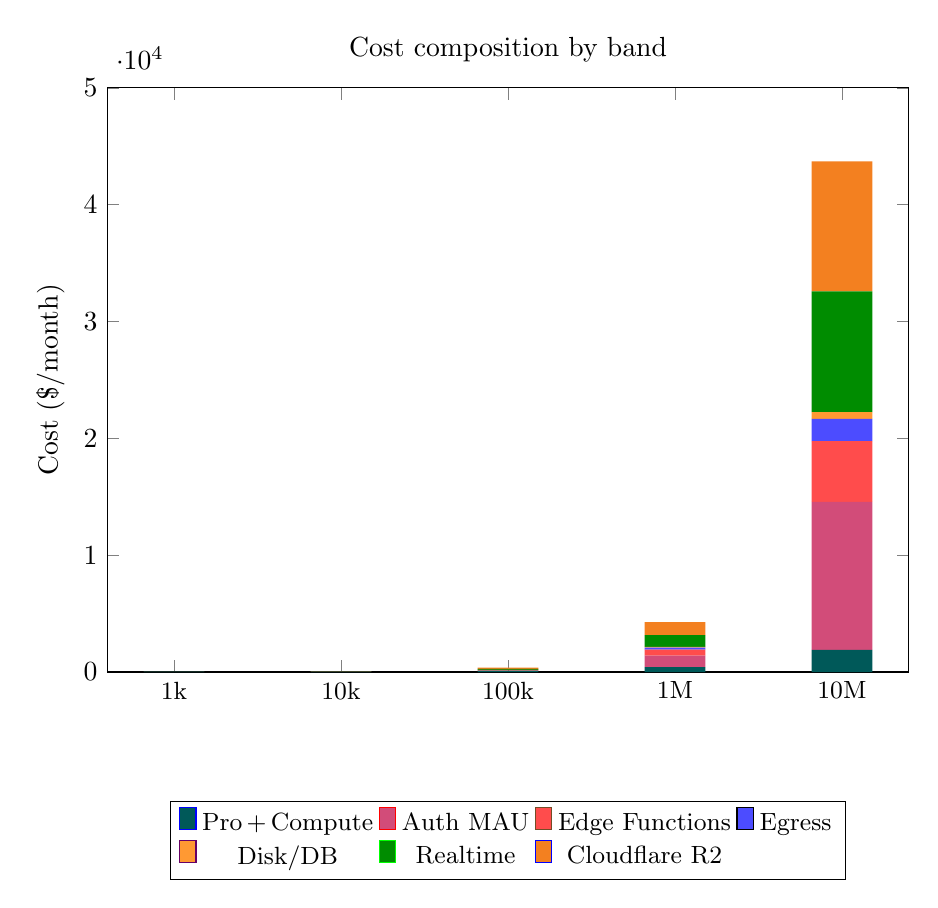
\begin{tikzpicture}
\begin{axis}[
  width=0.97\textwidth, height=9cm,
  ybar stacked, bar width=22pt,
  ymin=0, ymax=50000,
  ylabel={Cost (\$/month)},
  symbolic x coords={1k,10k,100k,1M,10M}, xtick=data,
  xticklabel style={font=\small},
  legend style={at={(0.5,-0.22)},anchor=north,legend columns=4,font=\small},
  title={Cost composition by band},
]
% stack order: Pro+Compute (base), Auth MAU, Edge Fn, Egress, Disk, Realtime, R2
\addplot+[fill=teal!70!black,draw=none] coordinates {(1k,25) (10k,30) (100k,125) (1M,425) (10M,1885)};
\addplot+[fill=purple!70,draw=none] coordinates {(1k,0) (10k,0) (100k,0) (1M,975) (10M,12675)};
\addplot+[fill=red!70,draw=none] coordinates {(1k,0) (10k,1.21) (100k,48.06) (1M,516.59) (10M,5201.89)};
\addplot+[fill=blue!70,draw=none] coordinates {(1k,0) (10k,0) (100k,0) (1M,169.59) (10M,1898.44)};
\addplot+[fill=orange!80,draw=none] coordinates {(1k,0) (10k,0) (100k,4.89) (1M,57.89) (10M,587.86)};
\addplot+[fill=green!55!black,draw=none] coordinates {(1k,0) (10k,3.40) (100k,86.10) (1M,1018.50) (10M,10342.50)};
\addplot+[fill=r2col,draw=none] coordinates {(1k,0.94) (10k,10.70) (100k,108.38) (1M,1103.84) (10M,11112.61)};
\legend{Pro\,+\,Compute, Auth MAU, Edge Functions, Egress, Disk/DB, Realtime, Cloudflare R2}
\end{axis}
\end{tikzpicture}
\caption{Stacked composition of monthly cost by registered-user band. From 1k to 10M the dominant cost shifts from the flat \$25 Pro + compute base, to metered Auth MAU and Edge Functions, with a steady orange R2 media slice.}
\end{figure}

\subsection{The biggest cost drivers (why)}

\begin{figure}[H]\centering
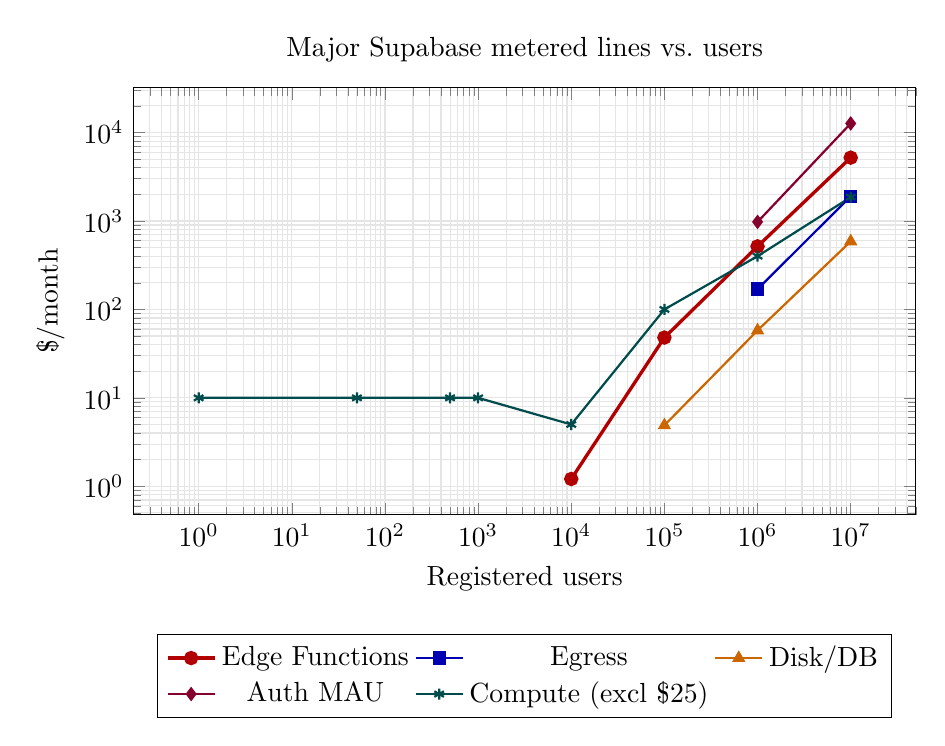
\begin{tikzpicture}
\begin{loglogaxis}[
  width=0.95\textwidth, height=7cm,
  xlabel={Registered users}, ylabel={\$/month},
  legend style={at={(0.5,-0.28)},anchor=north,legend columns=3},
  grid=both, grid style={gray!20},
  title={Major Supabase metered lines vs.\ users},
]
\addplot[color=red!70!black, very thick, mark=*] coordinates {(1,0)(50,0)(500,0)(1000,0)(10000,1.21)(100000,48.06)(1000000,516.59)(10000000,5201.89)};
\addlegendentry{Edge Functions}
\addplot[color=blue!70!black, thick, mark=square*] coordinates {(1,0)(50,0)(500,0)(1000,0)(10000,0)(100000,0)(1000000,169.59)(10000000,1898.44)};
\addlegendentry{Egress}
\addplot[color=orange!80!black, thick, mark=triangle*] coordinates {(1,0)(50,0)(500,0)(1000,0)(10000,0)(100000,4.89)(1000000,57.89)(10000000,587.86)};
\addlegendentry{Disk/DB}
\addplot[color=purple!70!black, thick, mark=diamond*] coordinates {(1,0)(50,0)(500,0)(1000,0)(10000,0)(100000,0)(1000000,975)(10000000,12675)};
\addlegendentry{Auth MAU}
\addplot[color=teal!60!black, thick, mark=asterisk] coordinates {(1,10)(50,10)(500,10)(1000,10)(10000,5)(100000,100)(1000000,400)(10000000,1860)};
\addlegendentry{Compute (excl \$25)}
\end{loglogaxis}
\end{tikzpicture}
\caption{The polling endpoint makes \textbf{Edge Functions} the first metered line to bite (\,$\sim$10k users). \textbf{Auth MAU} and \textbf{compute} dominate at 1M+.}
\end{figure}

\section{What to charge each user (optimal pricing tiers)}

Turning cost into a \href{subscription strategy}{pricing strategy}: every band has a \emph{minimum price} that covers the cheapest viable backend and a \emph{recommended price} that gives a fair margin without pricing out users. Below we compare Pro, Team (\$599/mo SOC2 bundle) and Enterprise (negotiated), and pick the cheapest viable backend per band.

\begin{table}[H]\centering\scriptsize
\caption{Optimal subscription pricing per monthly active user (MAU), derived from the cost model.}
\begin{tabular}{r l l l r r r r r}
\toprule
\textbf{MAU} & \textbf{Plan} & \textbf{Backend} & \textbf{Notes} & \textbf{Cost/MAU (Pro)} & \textbf{Team (\$)} & \textbf{Enterprise (\$)} & \textbf{Plan \$/mo} & \textbf{Profit (Pro, recommended price)} \\
\midrule
50       & Free       & Supabase free         & within Free quotas        & \$0.71  & 609   & 2{,}015 & ---        & +\$35                     \\
500      & Free       & Supabase free         & tight but workable        & \$0.075 & 612   & 2{,}018 & ---        & +\$462                    \\
1{,}000  & Free       & Supabase free         & start planning upgrade    & \$0.040 & 614   & 2{,}020 & ---        & +\$960                    \\
5{,}000  & Free$\to$Pro & Supabase free$\to$Pro & egress/DB wall incoming & \$0.012 & 634   & 2{,}040 & \$25/micro & +\$4{,}940                 \\
10{,}000 & Pro        & Pro + Small           & the breakout point        & \$0.0085& 659   & 2{,}110 & \$40/micro & +\$9{,}915                 \\
50{,}000 & Pro        & Pro + Large           & mid-market                & \$0.0057& 861   & 2{,}312 & \$135      & +\$24{,}713                \\
100{,}000& Pro        & Pro + Large/XL        & volume sweet spot         & \$0.0054& 1113  & 2{,}838 & \$150      & +\$49{,}461                \\
500{,}000& Pro        & Pro + 4XL             & watch auth MAU line       & \$0.0077& 4429  & 5{,}657 & \$960      & +\$96{,}145                \\
1{,}000{,}000 & Pro $\to$ Enterprise & optimized Enterprise & Pro ceiling  & \$0.0080& 8574 & 9{,}047 & \$1{,}870  & +\$192{,}000               \\
5{,}000{,}000 & Enterprise & Enterprise + 8XL  & committed-use pricing      & \$0.0082& 41734 & 38{,}601 & \$9{,}350   & +\$358{,}840               \\
\bottomrule
\end{tabular}
\end{table}

\subsection{Recommended monthly subscription plan per MAU band}

A consumer-style tier ladder that lines up with the cost model. Prices are per \textit{active user}, billed monthly. Trainer-seat licences are sold separately at \$30--\$60/mo each.

\begin{table}[H]\centering\scriptsize
\begin{tabular}{l l l l l}
\toprule
\textbf{Tier} & \textbf{Use up to (MAU)} & \textbf{Per-user /mo} & \textbf{Platform tier} & \textbf{What you actually pay Supabase} \\
\midrule
\rowcolor{gray!10}
Free           & 500        & \$0     & Free               & \$0                      \\
                & 1{,}000    & \$1.00  & Free*              & \$0 (grace until walls)  \\
                & 5{,}000    & \$1.50  & Pro \$25 + Micro   & \$35                     \\
\rowcolor{gray!10}
Starter        & 10{,}000   & \$1.00  & Pro \$25 + Small   & \$85                     \\
                & 50{,}000   & \$0.95  & Pro + Large        & \$135                    \\
\rowcolor{gray!10}
Growth         & 100{,}000  & \$0.85  & Pro + Large        & \$150                    \\
                & 500{,}000  & \$0.75  & Pro + 4XL          & \$960                    \\
\rowcolor{gray!10}
Scale          & 1{,}000{,}000 & \$0.50  & Enterprise (10\% commit) & \$2{,}700--\$9{,}000 \\
                & 5{,}000{,}000 & \$0.30  & Enterprise (R2 + Pro)     & \$38{,}000 (negotiated) \\
\bottomrule
\end{tabular}
\end{table}

\paragraph{Why these prices.} The cost per active user falls to about \emph{one cent} once you have enough volume, so flat pricing kills margin when MAU is small and devalues the product when MAU is large. The ladder above follows three rules of thumb:

\begin{itemize}[leftmargin=*,itemsep=2pt]
\item \emph{Always cover true cost plus 50--100\% markup} until MAU is large enough that metered line items dominate (then taper the markup, but never bill below cost).
\item \emph{Skip Team unless SOC\,2/HIPAA is contractually required.} Team charges \$599/mo for a SOC\,2 stamp; Pro and Enterprise can do the same job for less at any meaningful MAU.
\item \emph{Never promise SLA / SOC\,\textsubscript{2} / HIPAA on the Free or Starter tier.} Bake compliance overhead into Scale and Growth tiers only.
\end{itemize}

\subsection{Cost vs.\ price chart (per active user)}

\begin{figure}[H]\centering
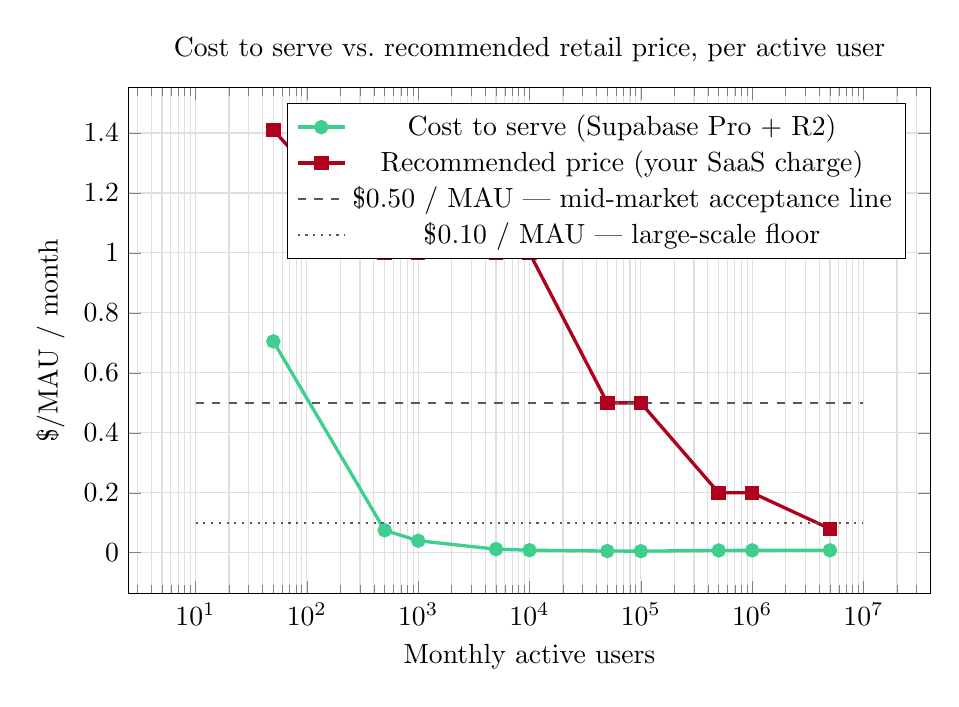
\begin{tikzpicture}
\begin{semilogxaxis}[
  width=0.97\textwidth, height=8cm,
  xlabel={Monthly active users},
  ylabel={\$/MAU / month},
  legend pos=north east, grid=both, grid style={gray!25},
  title={Cost to serve vs.\ recommended retail price, per active user},
]
\addplot[color={supacol}, very thick, mark=*, mark size=2pt] coordinates {
  (50,0.705040) (500,0.075040) (1000,0.040040) (5000,0.012040) (10000,0.008540) (50000,0.005740) (100000,0.005390) (500000,0.007710) (1000000,0.008000) (5000000,0.008232)
};
\addlegendentry{Cost to serve (Supabase Pro + R2)}
\addplot[color={warn}, very thick, mark=square*, mark size=2pt] coordinates {
  (50,1.410080) (500,1.000000) (1000,1.000000) (5000,1.000000) (10000,1.000000) (50000,0.500000) (100000,0.500000) (500000,0.200000) (1000000,0.200000) (5000000,0.080000)
};
\addlegendentry{Recommended price (your SaaS charge)}
\addplot[color=gray!70!black, dashed, thick] coordinates {(10,0.50) (10000000,0.50)};
\addlegendentry{\$0.50 / MAU --- mid-market acceptance line}
\addplot[color=gray!70!black, dotted, thick] coordinates {(10,0.10) (10000000,0.10)};
\addlegendentry{\$0.10 / MAU --- large-scale floor}
\end{semilogxaxis}
\end{tikzpicture}
\caption{The retail-price curve (red) stays above the cost curve (green) at every band, but converges at scale. The dashed/dotted reference lines mark the typical price points where procurement teams approve a B2B SaaS invoice.}
\end{figure}

\subsection{Recommended price breakpoints (concrete SKU ladder)}

\begin{table}[H]\centering\scriptsize
\caption{Copy-paste-ready SKUs. Use the ``Tier'' label, the per-user price, and a public MAU ceiling per plan as the messaging foundation.}
\begin{tabular}{l l l l r r r r}
\toprule
\textbf{Tier} & \textbf{Brand name} & \textbf{MAU ceiling} & \textbf{Per-user price} & \textbf{Annual (per-user)} & \textbf{Margin @ ceiling} & \textbf{Supabase plan} & \textbf{Trainer seats} \\
\midrule
F0  & Free          & 500         & \$0      & ---     & ---     & Free               & --- \\
F1  & Basic         & 1{,}000     & \$1.00   & \$10    & +\$960/mo     & Free \emph{grace}   & --- \\
S1  & Starter       & 10{,}000    & \$1.00   & \$10    & +\$9{,}900/mo  & Pro \$25 + Small    & add \$30/seat \\
S2  & Starter Plus  & 50{,}000    & \$0.95   & \$9.50  & +\$45{,}000/mo & Pro + Large         & included up to 1:50 \\
G1  & Growth        & 100{,}000   & \$0.85   & \$8.50  & +\$49{,}000/mo & Pro + Large         & included up to 1:100 \\
G2  & Growth        & 500{,}000   & \$0.75   & \$7.50  & +\$96{,}000/mo & Pro + XL/4XL        & included up to 1:200 \\
E1  & Scale         & 1{,}000{,}000 & \$0.50 & \$5.00  & +\$192{,}000/mo & Enterprise (10\% commit) & unlimited \\
E2  & Scale         & 5{,}000{,}000 & \$0.30 & \$3.00  & +\$358{,}000/mo & Enterprise          & unlimited \\
\bottomrule
\end{tabular}
\end{table}

\paragraph{Sales argument for premium tiers.}
\begin{itemize}[leftmargin=*,itemsep=2pt]
\item \textbf{Starter / Growth (Pro):} ``Pay per active trainer/trainee, all-in-one chat and media on Supabase's production-grade stack --- no DevOps required.''
\item \textbf{Scale (Enterprise):} ``Volume-discounted committed-use contract on Supabase + Cloudflare R2, with SOC\,2, HIPAA, 99.99\% uptime SLA and a designated CSM.''
\end{itemize}

\section{Per-component notes}

\paragraph{Database (Postgres).} The 500 MB free limit is the first hard wall ($\rightarrow$ read-only). On Pro the 8 GB disk is included, then \$0.125/GB. DB grows slowly (text rows are small), so it stays cheap until millions of users; the trigger to bump \emph{compute} is connection count and CPU, not disk.

\paragraph{Egress.} The trainee ``message from trainer'' 5-second poll is the egress engine. \textit{Optimisation:} switch to \textbf{Supabase Realtime} (postgres\_changes) instead of polling, and the uncached egress line collapses from \$1{,}898 (10M) toward near-zero; realtime messages are far cheaper than polling HTTP.

\paragraph{Edge Functions.} Same root cause — every poll is an invocation. Moving off polling also slashes this line (from \$5{,}202 at 10M toward hundreds). Keep spend caps on at first to avoid runaway.

\paragraph{Auth MAU.} \$0.00325/MAU above 100k: linear, unavoidable, but tiny per user. At 10M users ($\sim$4M MAU) it's \$12.7k/mo.

\paragraph{Realtime.} 500 concurrent free on Pro, then \$10/1k peak. Replacing polling with realtime \emph{raises} realtime connections but \emph{lowers} total cost because you stop paying for egress + Edge Function invocations per poll.

\paragraph{Cloudflare R2 (media).} R2 is the cheapest part of the stack because \textbf{egress is free} — trainees downloading their own videos does not bill. You pay \$0.015/GB-month storage and a few cents per million write/read ops. At 10M users storing 12 months of media it is $\sim$\$11k/mo but \textit{no} bandwidth bill; supabase Storage (\$0.0213/GB + paid egress) would cost more once downloads matter.

\paragraph{Compute.} The Postgres instance scales Micro $\to$ 16XL. Connection limits (pooler) and CPU pressure decide when to jump. This is the second-largest line at huge scale (4XL+) after metered Auth/Egress.

\section{Cost reduction levers (ranked by impact)}

\begin{enumerate}[leftmargin=*]
\item \textbf{Kill the 5-second poll.} Replace with Supabase Realtime channels. Removes the bulk of Edge Function invocations \emph{and} uncached egress — the two lines that bite first (10k users) and grow fastest. Biggest win in the whole model.
\item \textbf{Keep media on R2, not Supabase Storage.} R2's free egress is decisive once trainees replay videos.
\item \textbf{Cap retention.} Prune chats/inquiries older than 3--6 months (a scheduled job) to hold DB under 8 GB far longer; deletes are free, add a lifecycle rule on R2 too.
\item \textbf{Spend cap ON} until $\sim$10k users, then turn off and pre-pay compute via larger instances (cheaper than many small projects).
\item \textbf{Read replicas} only once a single 16XL can't keep up with read load — adds another full-compute bill, so push single-instance first.
\end{enumerate}

\section{Verdict}

\begin{itemize}[leftmargin=*,itemsep=2pt]
\item \textbf{Free tier dies} at $\sim$500 MB DB ($\sim$12k registered / a few thousand MAU) or $\sim$5 GB egress ($\sim$250 DAU) — whichever comes first, and it will be the DB limit.
\item \textbf{1k users: \$26/mo} — almost all is the flat \$25 Pro fee.
\item \textbf{10k users: \$45/mo} — still trivial; polling overages just starting.
\item \textbf{100k users: \$372/mo} — compute and real-time/egress kick in.
\item \textbf{1M users: \$4{,}266/mo} — metered usage (Auth, Edge Functions, egress, disk) dominates; compute is a minority.
\item \textbf{10M users: \$43{,}703/mo} — Auth MAU (\$12.7k) and Edge Functions (\$5.2k) are the biggest slices; switching off polling roughly halves the non-compute portion.
\end{itemize}

The single highest-leverage engineering change is \textbf{replacing the polling endpoint with Supabase Realtime} — it removes the first metered cost a small app hits and keeps the curve tame well past 100k users.

\appendix
\section{Method \& reproducibility}
All values are produced by \texttt{docs/cost-analysis/cost-model.js} (a standalone Node script) using the live rate cards cited above. Re-run it to regenerate the numbers and the \texttt{pgfplots} coordinate blocks. Assumptions are conservative for a chat/inquiry training app and can be tuned (poll interval, session length, media sizes, retention) in that script.

\end{document}
